% questions.tex —— 2006 年·普通高考·安徽卷文科 · 题目内容片段（无答案）
% 由 tools/generate_projects.py 依来源总账自 2006/2006_数学真题_安徽文_试题.md 生成，勿手改（改源 MD 后重跑）


\begin{gktip}
\textbf{来源及状态}：按本机固定 PDF 的两页题面转录，PDF 第 1、2 页印刷页码分别为 278、279；第二位复核者已逐栏对照全部 22 题，源内疑点仍待核。固定副本的出版者、版次、来源链和官方身份均未核；本卷已与该副本作本库内部绑定，该关系不认证官方来源。源文件只见题面，未见答案、解析、题目分值或总分。三幅题图已按源图矢量重绘、局部编译并独立对照，正式排版验收尚未完成。

\textbf{源页定位}：PDF 第 1 页含第 1–19 题，第 9 题图在左栏、选项延续到中栏，第 19 题图在右栏；第 2 页含第 20–22 题，第 22 题图在右栏。

\textbf{待核}：第 2 题四个选项与题面不等式的解集不匹配；第 5 题固定副本中“椭圆”后只见 $\dfrac{x^2}{6}+\dfrac{y^2}{2}$，未见等号及右侧。均保留固定副本可见内容，不推定正式原卷同样如此。
\end{gktip}

\gkpart{一、选择题}

\begin{question}
\gkti{1}设全集 $U=\{1,2,3,4,5,6,7,8\}$，集合 $S=\{1,3,5\}$，$T=\{3,6\}$，则 $\complement_U(S\cup T)$ 等于\mbox{（　　）}

（A）$\varnothing$　（B）$\{2,4,7,8\}$　（C）$\{1,3,5,6\}$　（D）$\{2,4,6,8\}$

\end{question}
\begin{question}
\gkti{2}不等式 $\dfrac1x<\dfrac12$ 的解集是\mbox{（　　）}

（A）$(-\infty,2)$　（B）$(2,+\infty)$　（C）$(0,2)$　（D）$(-\infty,2)\cup(2,+\infty)$

\begin{gktip}
待核（ISSUE-1216）：固定副本所印四个选项与该不等式的解集不匹配；不据此改写选项。
\end{gktip}

\end{question}
\begin{question}
\gkti{3}函数 $y=\mathrm e^{x+1}$（$x\in\mathbb R$）的反函数是\mbox{（　　）}

（A）$y=1+\ln x$（$x>0$）　（B）$y=1-\ln x$（$x>0$）

（C）$y=-1-\ln x$（$x>0$）　（D）$y=-1+\ln x$（$x>0$）

\end{question}
\begin{question}
\gkti{4}“$x>3$”是“$x^2>4$”的\mbox{（　　）}

（A）必要不充分条件　（B）充分不必要条件　（C）充分必要条件　（D）既不充分也不必要条件

\end{question}
\begin{question}
\gkti{5}若抛物线 $y^2=2px$ 的焦点与椭圆 $\dfrac{x^2}{6}+\dfrac{y^2}{2}$ 的右焦点重合，则 $p$ 的值为\mbox{（　　）}

（A）$-2$　（B）$2$　（C）$-4$　（D）$4$

\begin{gktip}
待核（ISSUE-1217、ISSUE-1218）：固定副本中的椭圆式未见等号及右侧；本稿未补写。
\end{gktip}

\end{question}
\begin{question}
\gkti{6}表面积为 $2\sqrt3$ 的正八面体的各个顶点都在同一球面上，则此球的体积为\mbox{（　　）}

（A）$\dfrac{\sqrt2}{3}\pi$　（B）$\dfrac13\pi$　（C）$\dfrac23\pi$　（D）$\dfrac{2\sqrt2}{3}\pi$

\end{question}
\begin{question}
\gkti{7}直线 $x+y=1$ 与圆 $x^2+y^2-2ay=0$（$a>0$）没有公共点，则 $a$ 的取值范围是\mbox{（　　）}

（A）$(0,\sqrt2-1)$　（B）$(\sqrt2-1,\sqrt2+1)$　（C）$(-\sqrt2-1,\sqrt2+1)$　（D）$(0,\sqrt2+1)$

\end{question}
\begin{question}
\gkti{8}对于函数 $f(x)=\dfrac{\sin x+1}{\sin x}$（$0<x<\pi$），下列结论正确的是\mbox{（　　）}

（A）有最大值而无最小值　（B）有最小值而无最大值

（C）有最大值且有最小值　（D）既无最大值又无最小值

\Needspace{0.4\textheight}
\end{question}
\begin{question}
\gkti{9}将函数 $y=\sin\omega x$（$\omega>0$）的图象按向量 $\vec a=\left(-\dfrac\pi6,0\right)$ 平移，平移后的图象如图所示，则平移后的图象所对应的函数解析式是\mbox{（　　）}

（A）$y=\sin\left(x+\dfrac\pi6\right)$　（B）$y=\sin\left(x-\dfrac\pi6\right)$

（C）$y=\sin\left(2x+\dfrac\pi3\right)$　（D）$y=\sin\left(2x-\dfrac\pi3\right)$
\nopagebreak[4]
\begin{center}% 2006 安徽文科 Q9；函数与标注按固定来源重绘。
\begin{tikzpicture}[x=1.45cm,y=0.95cm,line cap=round,line join=round,>=stealth,font=\small]
  \draw[->] (-0.9,0) -- (3.4,0) node[right] {$x$};
  \draw[->] (0,-1.5) -- (0,1.65) node[above] {$y$};
  \draw[thick,domain=-0.8:3.0,samples=140] plot (\x,{sin(deg(2*\x+pi/3))});
  \draw[dashed] ({7*pi/12},0) -- ({7*pi/12},-1) -- (0,-1);
  \node[below right] at (0,0) {$O$};
  \node[left] at (0,1) {$1$};
  \node[left] at (0,-1) {$-1$};
  \node[above] at ({7*pi/12},0) {$\dfrac{7\pi}{12}$};
\end{tikzpicture}
\end{center}
\nopagebreak[4]
\end{question}
\begin{question}
\gkti{10}如果实数 $x,y$ 满足条件
\nopagebreak[4]
\[
\begin{cases}
x-y+1\geqslant0,\\
y+1\geqslant0,\\
x+y+1\leqslant0,
\end{cases}
\]
那么 $2x-y$ 的最大值为\mbox{（　　）}

（A）$2$　（B）$1$　（C）$-2$　（D）$-3$

\end{question}
\begin{question}
\gkti{11}如果 $\triangle A_1B_1C_1$ 的三个内角的余弦值分别等于 $\triangle A_2B_2C_2$ 的三个内角的正弦值，则\mbox{（　　）}

（A）$\triangle A_1B_1C_1$ 和 $\triangle A_2B_2C_2$ 都是锐角三角形

（B）$\triangle A_1B_1C_1$ 和 $\triangle A_2B_2C_2$ 都是钝角三角形

（C）$\triangle A_1B_1C_1$ 是钝角三角形，$\triangle A_2B_2C_2$ 是锐角三角形

（D）$\triangle A_1B_1C_1$ 是锐角三角形，$\triangle A_2B_2C_2$ 是钝角三角形

\end{question}
\begin{question}
\gkti{12}在正方体上任选 3 个顶点连成三角形，则所得的三角形是直角非等腰三角形的概率为\mbox{（　　）}

（A）$\dfrac17$　（B）$\dfrac27$　（C）$\dfrac37$　（D）$\dfrac47$

\end{question}
\gkpart{二、填空题}

\begin{question}
\gkti{13}设常数 $a>0$，$\left(ax^2+\dfrac1{\sqrt x}\right)^4$ 展开式中 $x^3$ 的系数为 $\dfrac32$，则 $a=$ \gkblank{}。

\end{question}
\begin{question}
\gkti{14}在平行四边形 $ABCD$ 中，$\overrightarrow{AB}=\vec a$，$\overrightarrow{AD}=\vec b$，$\overrightarrow{AN}=3\overrightarrow{NC}$，$M$ 为 $BC$ 的中点，则 $\overrightarrow{MN}=$ \gkblank{}。（用 $\vec a,\vec b$ 表示）

\end{question}
\begin{question}
\gkti{15}函数 $f(x)$ 对于任意实数 $x$ 满足条件 $f(x+2)=\dfrac1{f(x)}$，若 $f(1)=-5$，则 $f(f(5))=$ \gkblank{}。

\end{question}
\begin{question}
\gkti{16}平行四边形的一个顶点 $A$ 在平面 $\alpha$ 内，其余顶点在 $\alpha$ 的同侧，已知其中两个顶点到 $\alpha$ 的距离分别为 $1,2$，那么剩下的一个顶点到平面 $\alpha$ 的距离可能是：① $1$；② $2$；③ $3$；④ $4$。

以上结论正确的是 \gkblank{}。（写出所有正确结论的编号）

\end{question}
\gkpart{三、解答题}

\begin{question}
\gkti{17}已知 $0<\alpha<\dfrac\pi2$，$\sin\alpha=\dfrac45$。

（1） 求 $\dfrac{\sin^2\alpha+\sin2\alpha}{\cos^2\alpha+\cos2\alpha}$ 的值；

（2） 求 $\tan\left(\alpha-\dfrac{5\pi}{4}\right)$ 的值。

\end{question}
\begin{question}
\gkti{18}在添加剂的搭配适用中，为了找到最佳的搭配方案，需要对各种不同的搭配方式作比较，在试制某种牙膏新品种时，需要选用两种不同的添加剂。现有芳香度分别为 $0,1,2,3,4,5$ 的六种添加剂可供选用。根据试验设计学原理，通常首先要随机选取两种不同的添加剂进行搭配试验。

（1） 求所选用的两种不同的添加剂的芳香度之和等于 $4$ 的概率；

（2） 求所选用的两种不同的添加剂的芳香度之和不小于 $3$ 的概率。

\Needspace{0.4\textheight}
\end{question}
\begin{question}
\gkti{19}如图，$P$ 是边长为 $1$ 的正六边形 $ABCDEF$ 所在平面外一点，$PA=1$，$P$ 在平面 $ABC$ 内的射影为 $BF$ 的中点 $O$。

（1） 证明：$PA\perp BF$；

（2） 求面 $APB$ 与面 $DPB$ 所成二面角的大小。
\nopagebreak[4]
\begin{center}% 2006 安徽文科 Q19；仿射投影为示意，O 为 BF 中点。
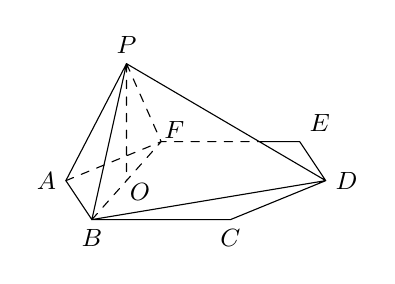
\begin{tikzpicture}[scale=1.1,line cap=round,line join=round,font=\small]
  \coordinate (A) at (0,0);
  \coordinate (B) at (0.3,-0.45);
  \coordinate (C) at (1.9,-0.45);
  \coordinate (D) at (3,0);
  \coordinate (E) at (2.7,0.45);
  \coordinate (F) at (1.1,0.45);
  \coordinate (H) at (2.2333333,0.45); % PD 与 FE 的投影交点，不标为题设点
  \coordinate (O) at (0.7,0);
  \coordinate (P) at (0.7,1.35);
  \draw[dashed] (A)--(F)--(H) (B)--(F) (P)--(F) (P)--(O);
  \draw (H)--(E) (A)--(B)--(C)--(D)--(E) (B)--(D) (P)--(A) (P)--(B) (P)--(D);
  \node[left] at (A) {$A$};
  \node[below] at (B) {$B$};
  \node[below] at (C) {$C$};
  \node[right] at (D) {$D$};
  \node[above right] at (E) {$E$};
  \node[above right,inner sep=1pt] at (F) {$F$};
  \node[below right,inner sep=1pt] at (O) {$O$};
  \node[above] at (P) {$P$};
\end{tikzpicture}
\end{center}
\nopagebreak[4]
\end{question}
\begin{question}
\gkti{20}设函数 $f(x)=x^3+bx^2+cx$（$x\in\mathbb R$），已知 $g(x)=f(x)-f'(x)$ 是奇函数。

（1） 求 $b,c$ 的值；

（2） 求 $g(x)$ 的单调区间与极值。

\end{question}
\begin{question}
\gkti{21}在等差数列 $\{a_n\}$ 中，$a_1=1$，前 $n$ 项和 $S_n$ 满足条件 $\dfrac{S_{2n}}{S_n}=\dfrac{4n+2}{n+1}$，$n=1,2,\cdots$。

（1） 求数列 $\{a_n\}$ 的通项公式；

（2） 记 $b_n=a_np^{a_n}$（$p>0$），求数列 $\{b_n\}$ 的前 $n$ 项和 $T_n$。

\Needspace{0.4\textheight}
\end{question}
\begin{question}
\gkti{22}如图，$F$ 为双曲线 $C:\dfrac{x^2}{a^2}-\dfrac{y^2}{b^2}=1$（$a>0,b>0$）的右焦点，$P$ 为双曲线 $C$ 右支上一点，且位于 $x$ 轴上方，$M$ 为左准线上一点，$O$ 为坐标原点。已知四边形 $OFPM$ 为平行四边形，$|PF|=\lambda|OF|$。

（1） 写出双曲线 $C$ 的离心率 $e$ 与 $\lambda$ 的关系式；

（2） 当 $\lambda=1$ 时，经过焦点 $F$ 且平行于 $OP$ 的直线交双曲线于 $A,B$ 点，若 $|AB|=12$，求此时的双曲线方程。
\nopagebreak[4]
\begin{center}% 2006 安徽文科 Q22；取 a=1、e=2 作示意，P 在右支且 y>0。
\begin{tikzpicture}[x=0.9cm,y=0.72cm,line cap=round,line join=round,>=stealth,font=\small]
  \coordinate (O) at (0,0);
  \coordinate (F) at (2,0);
  \coordinate (M) at (-0.5,{sqrt(15)/2});
  \coordinate (P) at (1.5,{sqrt(15)/2});
  \draw[->] (-3.4,0)--(3.5,0) node[right] {$x$};
  \draw[->] (0,-3.7)--(0,3.9) node[above] {$y$};
  \draw (-0.5,-3.1)--(-0.5,3.1);
  \draw[thick,domain=-3.4:3.4,samples=100] plot ({sqrt(1+\x*\x/3)},\x);
  \draw[thick,domain=-3.4:3.4,samples=100] plot ({-sqrt(1+\x*\x/3)},\x);
  \draw (O)--(M)--(P)--(F);
  \node[below right] at (O) {$O$};
  \node[below] at (F) {$F$};
  \node[left] at (M) {$M$};
  \node[above left] at (P) {$P$};
\end{tikzpicture}
\end{center}
\nopagebreak[4]

\end{question}